\chapter{Particle-in-Cell Simulations}

\label{ch:particle_in_cell}


Plasmas are complex non-linear systems and contain many unknown variables. Therefore, simplified models are often used to capture major physics of the system whist ignoring details that can be considered negligible. There are several types of plasma models but the most commonly used methods are fluid description models and kinetic description models \cite{Kim2005}. 

The fluid description method aims to generalise the plasma quantities, such as its density and velocity, by averaging them over a 2D or 3D region . This is achieved by numerically solving the fluid equations; obtained by utilising the velocity components of the Boltzmann equation \cite{Kim2005}. Then, the electromagnetic fields are obtained by combining the fluid equations with Maxwell's equations. 

In contrast, kinetic description models track the position and velocities of particles within the plasma, taking into account the electromagnetic forces acting on them. As a general rule of thumb, fluid models simulate the plasma behaviour over a macroscopic scale; whilst kinetic models highlight plasma behaviour at the microscopic level.

Particle-in-cell (PIC) simulations are a variant of kinetic description models that tend to be favoured because of its easy formulation. Real-world plasma systems contain a prodigious number of particles, which include electrons, ions, and the background neutral gas; thus, tracking all these particles would be immensely computationally taxing. PIC simulations partially solve this by tracking so-called \textit{super-particles} \cite{Tskhakaya2007}. Each super-particle is scaled to represent a number of ``real" particles. This scaling factor does not affect the trajectory of the super-particles as the motion of particles within a electromagnetic field are only governed by its mass to charge ratio (see the Newton-Lorentz expression in equation \ref{eq:newton_lorentz}) \cite{Tskhakaya2007}. For the rest of this chapter, the term super-particle and particles are used interchangeably.

The PIC simulations discussed in this report are known as 2D-3v simulations, i.e. they are 2-dimensional in space but 3-dimensional in velocity. In these simulations, the particle properties (i.e. their position an velocity) are defined in continuous space within the simulation domain. However, the electromagnetic field values are only specified at fixed grid points. Therefore, intermediary steps are required to discretise charges and current densities onto the grid and also interpolation of forces by fields on the particles. These particles and fields are updated sequentially, with time being advanced in small discrete constant steps. An overview of this procedure can be seen in figure \ref{fig:pic_flowchart} \cite{Birdsall1991}. The rest of this chapter is dedicated to providing an overview of each process in the flow chart.

\begin{figure}[h!]
	\centering
	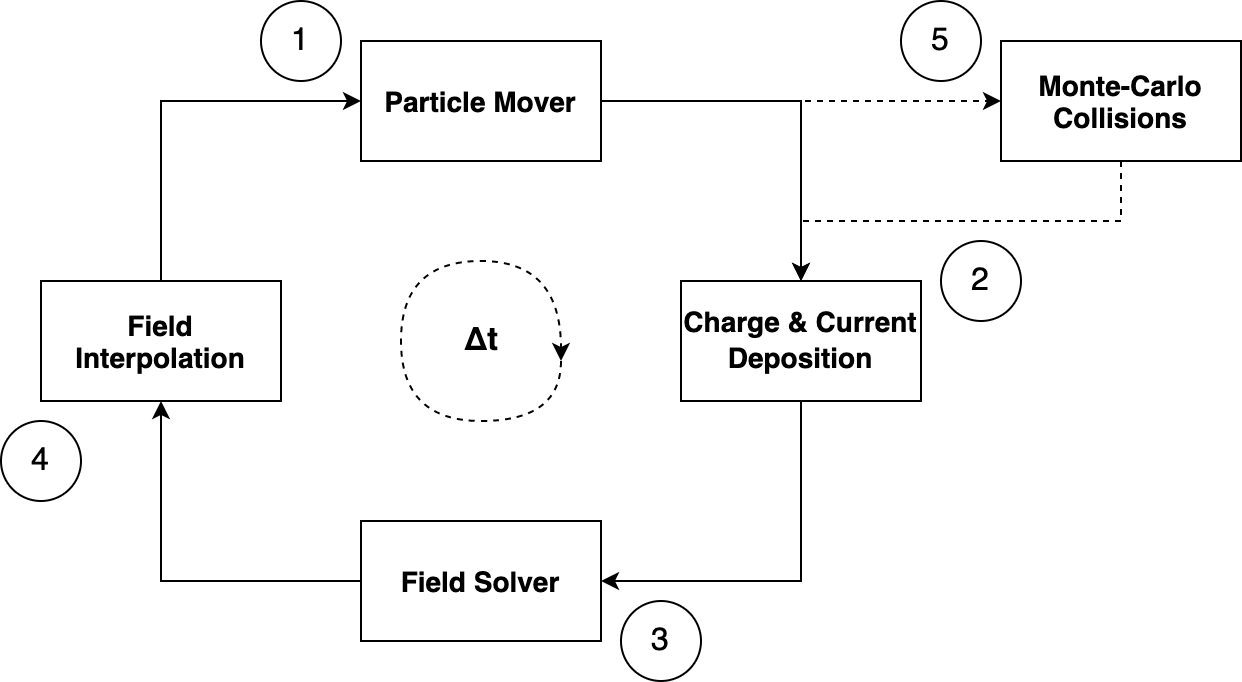
\includegraphics[width=\linewidth]{particle_in_cell/figures/pic_flowchart.png}
	\caption{Process flow of PIC simulations.}
	\label{fig:pic_flowchart}
\end{figure} 


\section{Particle Mover}

When first launching the PIC simulation, a random distribution of particle positions and velocities is initialised within the simulation domain. The acceleration of a particle is given by Newton's second law:
\begin{equation}
	\frac{d\bm{v}}{dt} = \frac{F}{m}
	\label{eq:acceleration}
\end{equation}

The force acting on the particle is determined by the Lorentz force:
\begin{equation}
	F = q(\bm{E} + \bm{v} \times \bm{B)}
	\label{eq:lorentz_force}
\end{equation}

where $\bm{E}$ and $\bm{B}$ are the electric and magnetic fields respectively, and $q$ corresponds to the charge of the particle.

Combining equations \ref{eq:acceleration} and \ref{eq:lorentz_force} gives the Newton-Lorentz equation:
\begin{equation}
	\frac{d\bm{v}}{dt} = \frac{q}{m}(\bm{E} + \bm{v} \times \bm{B)}
	\label{eq:newton_lorentz}
\end{equation}

As for the particles velocity, it is given by: 
\begin{equation}
	\frac{d\bm{s}}{dt} = \bm{v}
	\label{eq:velocity}
\end{equation}

In order to obtain the particle velocity and position, equations \ref{eq:newton_lorentz} and \ref{eq:velocity} have to be numerically integrated with respect to time using the \textit{finite-difference method}; specifically the \textit{leapfrog method} \cite{Hockney1988}. Thus, the new finite-difference forms of the respective equations are:

\begin{equation}
	\frac{\bm{v^{t + \frac{1}{2}}} - \bm{v^{t - \frac{1}{2}}}}{dt} = \frac{q}{m}(\bm{E} + (\frac{\bm{v^{t + \frac{1}{2}}} - \bm{v^{t - \frac{1}{2}}}}{2}) \times \bm{B)}
	\label{eq:newton_lorentz_finite_difference}
\end{equation}

\begin{equation}
	\frac{\bm{s^{t + 1}} - \bm{s^t}}{dt} = \bm{v^{t + \frac{1}{2}}}
	\label{eq:velocity_finite_difference}
\end{equation}

\begin{figure}[h!]
	\centering
	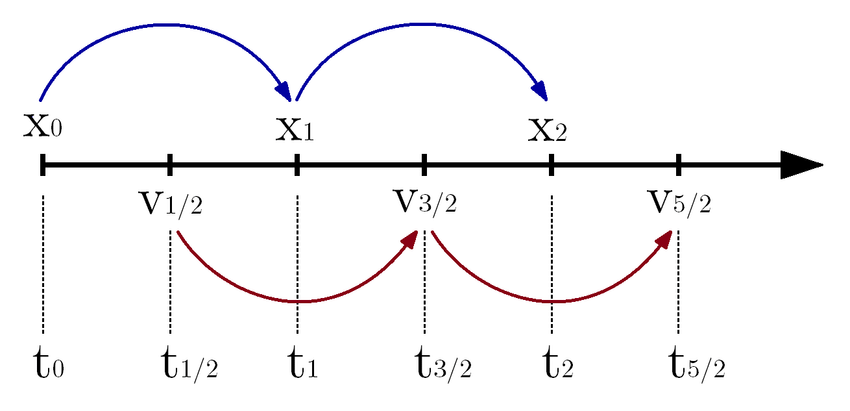
\includegraphics[width=0.6\linewidth]{particle_in_cell/figures/leap_frog.png}
	\caption{Illustration of forward-difference and central-difference form \cite{gisbert_piovella_2020}.}
	\label{fig:leap_frog}
\end{figure} 

Notice that the particle position is given by the \textit{forward-difference form}, whereas its velocity is given by the \textit{central-difference form}. This is done to conserve the energy of the dynamic system. An intuitive explanation for this is that when solving for the updated position of the particle, its average velocity should be used. Using either the initial or final velocities can result in the particle gaining energy if its accelerating, or losing energy if its decelerating. A visualisation of the difference can be seen in figure \ref{fig:leap_frog}. 

To solve the Newton-Lorentz equation, the de-facto method used is the \textit{Boris algorithm} \cite{Birdsall2004} for its accuracy, speed, and simplicity. The method first redefines both velocity terms as:
\begin{equation}
	\bm{v^{t - \frac{1}{2}}} = \bm{v^-} - \frac{q\bm{E}}{m}\frac{dt}{2}
	\label{eq:boris_electric_1}
\end{equation}
\begin{equation}
	\bm{v^{t + \frac{1}{2}}} = \bm{v^+} + \frac{q\bm{E}}{m}\frac{dt}{2}
	\label{eq:boris_electric_2}
\end{equation}

When substituted back into the the finite-difference Newton-Lorentz equation (equation \ref{eq:newton_lorentz_finite_difference}), this eliminates the electric field, resulting in an equation that expresses the rotation of the particle's velocity:

\begin{equation}
	\frac{\bm{v^+} - \bm{v^-}}{\Delta t} = \frac{q}{2m} (\bm{v^+} + \bm{v^-}) \times \bm{B}
\end{equation}

Because it describes a rotation, it can be solved geometrically. Using the following 2D case seen in figure \ref{fig:boris_rotation}, it can be determined that the angle through which the velocity rotates is:

\begin{equation}
	tan \left(\frac{\theta}{2} \right) = \frac{\bm{v^+} - \bm{v^-}}{\bm{v^+} + \bm{v^-}} = \frac{q\bm{B}}{m} \frac{\Delta t}{2}
\end{equation}

\begin{figure}[b!]
	\centering
	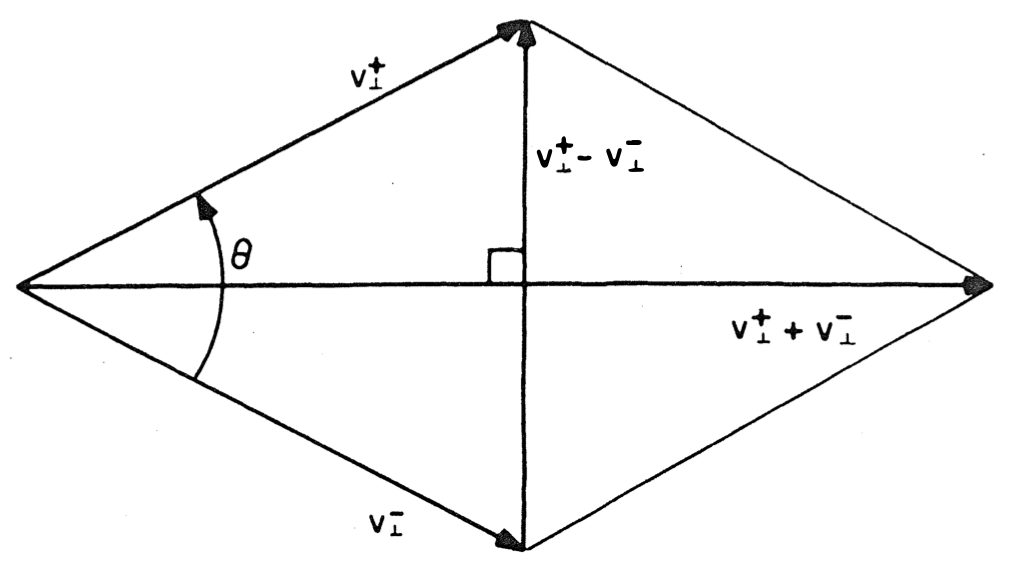
\includegraphics[width=0.6\linewidth]{particle_in_cell/figures/boris_rotation.png}
	\caption{Visualisation of velocity rotation from the Boris algorithm \cite{Birdsall2004}.}
	\label{fig:boris_rotation}
\end{figure} 

This angle can also be represented in vector form, referred to as $\bm{T}$. Using this vector form, a bisecting vector $\bm{v'}$ can be obtained is parallel to the $\bm{v^+} + \bm{v^-}$ vector (the sum of the pre-rotation and post-rotation vector), and perpendicular to both the $\bm{T}$ vector (the scaled magnetic field) and the $\bm{v^+} - \bm{v^-}$ vector (the difference between the post-rotational and pre-rotational velocity). 

\begin{equation}
	\bm{v'} = \bm{v^-} + \bm{v^-} \times \bm{T}
	\label{eq:boris_magnetic_1}
\end{equation}

Finally to obtain the $\bm{v^+} - \bm{v^-}$ vector, this intermediate vector $\bm{v'}$ is combined with a new vector $\bm{S}$ which can be thought of as a scaled version of vector $\bm{T}$ seen in equation \ref{eq:vector_S}. 

\begin{equation}
	\bm{v+} = \bm{v^-} + \bm{v'} \times \bm{S}
	\label{eq:boris_magnetic_2}
\end{equation}
\begin{equation}
	\bm{S} = \frac{2\bm{T}}{1 + \bm{T}^2}
	\label{eq:vector_S}
\end{equation}

Thus, in order to determine the new velocity of the particle:

\begin{enumerate}
	\item First calculate the velocity of the particle over the first half time step using equation \ref{eq:boris_electric_1}.
	\item Then perform the full rotation of the velocity due to the magnetic field using equations \ref{eq:boris_magnetic_1} and \ref{eq:boris_magnetic_2}.
	\item Finally, calculate the velocity of the particle over the second half time step using equation \ref{eq:boris_electric_2}.
\end{enumerate}

To obtain the particles new position, substitute the newly calculated velocity of the particle into equation \ref{eq:velocity_finite_difference}. Once calculated, the positions of each particle in the simulation can be updated.


\section{Charge and Current Deposition}

Once the particles have been moved, their charge and current densities are discretised onto a the specified grid. The exact method of discretising these properties depends on the type of grid for the PIC simulation. The one described in this report is for a uniform 2D rectilinear grid, known as  \textit{bilinear interpolation} \cite{Press1988C3}. 

\begin{figure}[h!]
	\centering
	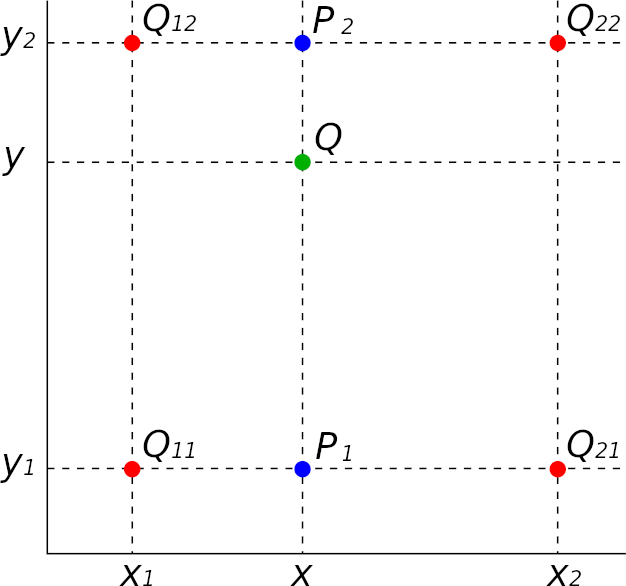
\includegraphics[width=0.55\linewidth]{particle_in_cell/figures/bilinear_interpotation_to_particle.png}
	\caption{Interpolation from the grid to the particles \cite{Ha2019}.}
	\label{fig:bilinear_interpotation_to_particle}
\end{figure} 

Consider the following case in figure \ref{fig:bilinear_interpotation_to_particle}. The charge of the particle within the grid cell is distributed across the four vertices of the cell, called the \textit{nodes}. The total charge experienced by each node must equal to the charge of the particle, with nodes closest to the particle experiencing the greatest weight. This can be expressed as:

\begin{equation}
\begin{aligned}
	Q_{11} = Q\frac{(x_2 - x) (y_2 - y)}{(x_2 - x_1) (y_2 - y_1)} \\
	Q_{12} = Q\frac{(x_2 - x) (y - y_1)}{(x_2 - x_1) (y_2 - y_1)} \\
	Q_{21} = Q\frac{(x - x_1) (y_2 - y)}{(x_2 - x_1) (y_2 - y_1)} \\
	Q_{22} = Q\frac{(x - x_1) (y - y_1)}{(x_2 - x_1) (y_2 - y_1)}
\end{aligned}
\end{equation}

Intuitively, the weight of a node corresponds to the ratio of the area of the rectangle opposite (formed by the point of the particle and the point of the opposite node) and the total area of the cell. 

Once the (weighted) charges at each node point has been calculated for all particles, the charge density of a node can be determined by summing the total charge on the node from all particles, then dividing by the area of the cell. This node area is typically given as $(x_2 - x_1) (y_2 - y_1)$, with the exception being nodes at the edges or corners of the simulation domain. With such cases, the resulting area is halved and quartered respectively.  

A similar process is done to determine the current densities around a node. However, rather than just summing the charges, the total sum of the product between the particles charge and average velocity are taken.


\section{Field Solver}

The field solver utilises the charge and current densities at the grid points to determine their corresponding electric and magnetic field values by solving Maxwell's equations. This report will only consider the electrostatic case and therefore will focus on the process of computing the electric field values. 

Gauss's law dictates that the divergence of the electric field in a region is proportional to its charge density:

\begin{equation}
	\nabla E = \frac{\rho}{\varepsilon_0}
\end{equation}

The electric field is determined as the gradient of the electric potential, and by substituting that into the above equation results in Poisson's equation:

\begin{equation}
	-\nabla^2 \phi = \frac{\rho}{\varepsilon_0}
\end{equation}

Considering a 2D case with a cartesian coordinate system, Poisson's equation can be rewritten as:

\begin{equation}
	\frac{\partial ^2 \phi}{\partial x^2} + \frac{\partial^2 \phi}{\partial y^2} = -\frac{\rho}{\varepsilon_0}
\end{equation}

In order to solve Poisson's equation in a discretised domain, the finite-difference method is employed. Specifically using the central-difference, the resulting approximation seen in equation \ref{eq:poisson_equation_finite_difference_no_diffusion} is produced, which is classed as second order accurate. 

\begin{equation}
	\frac{\phi_{x + \Delta x, y} - 2\phi_{x,y} + \phi_{x - \Delta x, y}}{\Delta x^2} + \frac{\phi_{x, y + \Delta y} - 2\phi_{x,y} + \phi_{x, y - \Delta y}}{\Delta y^2} = -\frac{\rho}{\varepsilon_0}
	\label{eq:poisson_equation_finite_difference_no_diffusion}
\end{equation}

There are several method to solve such an equation numerically. An overview of method used by XOOPIC (simulation program used in this work, see chapter 4) is described below. 

The Poisson equation is classed as an elliptic partial differential equation, which can be written in this form \cite{Press1988C19}:
\begin{equation}
	\mathcal{L}u = \lambda
\end{equation}
where $\mathcal{L}$ is the elliptical operator and $\lambda$ is the source term.

It is then possible to rewrite this as a diffusion equation (i.e. with respect to time):
\begin{equation}
	\frac{\partial u}{\partial t} = \frac{\partial^2 u}{\partial x^2} +\frac{\partial^2 u}{\partial y^2} - \lambda
	\label{eq:diffusion_equation}
\end{equation}
which is equivalent since as $t \to \infty$, $\frac{\partial u}{\partial t} \to 0$.

Therefore, equation \ref{eq:diffusion_equation} can be expressed as a diffusion equation in the finite-difference form:
\begin{equation}
	\frac{\phi_{x, y}^{t + \Delta t} - \phi_{x, y}^t}{\Delta t} = \frac{\phi_{x + \Delta x, y} - 2\phi_{x,y} + \phi_{x - \Delta x, y}}{\Delta x^2} + \frac{\phi_{x, y + \Delta y} - 2\phi_{x,y} + \phi_{x, y - \Delta y}}{\Delta y^2} + \frac{\rho}{\varepsilon_0}
	\label{eq:poisson_equation_finite_difference}
\end{equation}

From this, a technique known as the \textit{alternating-direction implicit} (ADI) method can be employed. In essence, the ADI method utilises a concept known as operator splitting, wherein the $\frac{\partial^2 \phi}{\partial x^2}$ and $\frac{\partial^2 \phi}{\partial y^2}$ terms can be decoupled, then each can be solved by iterating over half a time step. So for the first half time step, a pass is performed along the $x$ direction; then at the second half time step, a pass is performed along the $y$ direction as illustrated in figure \ref{fig:adi}. 

\begin{figure}[h!]
	\centering
	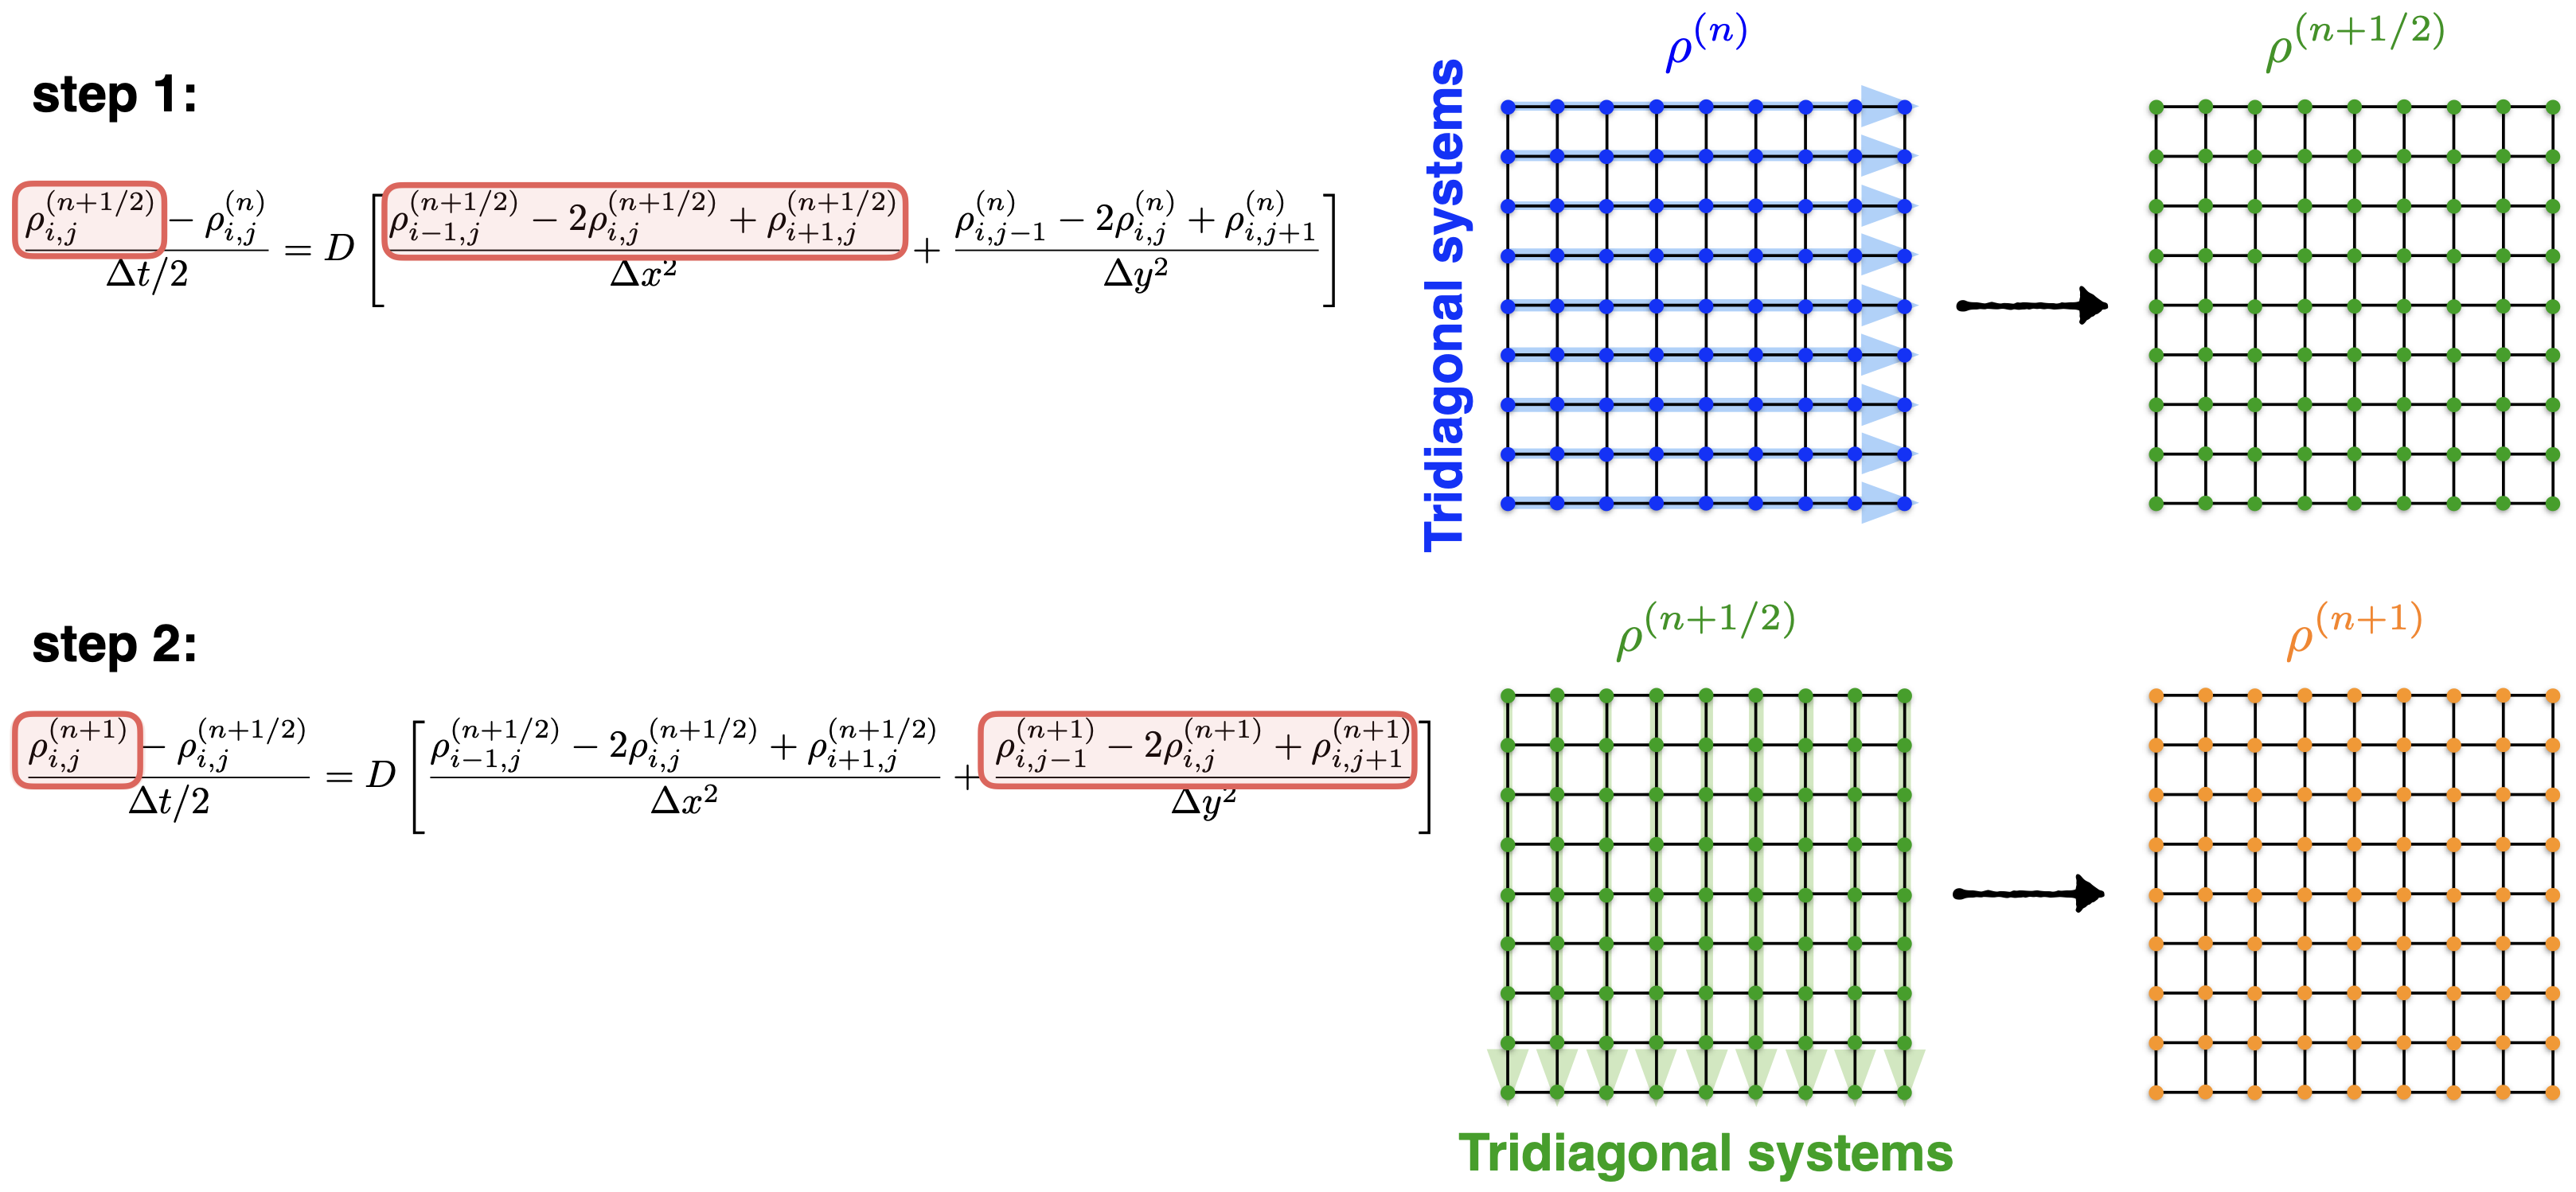
\includegraphics[width=\linewidth]{particle_in_cell/figures/adi.png}
	\caption{Illustration of ADI method \cite{Wermelinger}.}
	\label{fig:adi}
\end{figure} 

The benefit of this method is that rather than solving a large sparse matrix of a 2D system, a set of two independent 1D systems can be solved. These 1D systems can be arranged as a tridiagonal matrix, which can be efficiently solved using the \textit{Thomas algorithm} \cite{Press1988C1}. 

Once the Poisson equation is solved and the potentials at the grid determined, the electric field can be calculated again by the finite difference method. As the electric field is a vector, it needs to be calculated both along the direction of the $x$-axis and $y$-axis. Considering only the direction along the $x$-axis, equation \ref{eq:electric_field_equation} can be used. For the case of a boundary, equation \ref{eq:electric_field_equation_boundary} should be used instead.

\begin{equation}
	E_{x}^{i,j} = \frac{\phi_{i + \Delta x, j} - \phi_{i - \Delta x, j}}{2 \Delta x}
	\label{eq:electric_field_equation}
\end{equation}

\begin{equation}
	E_{x}^{i,j} = \frac{\phi_{i + \Delta x, j} - \phi_{i, j}}{\Delta x}
	\label{eq:electric_field_equation_boundary}
\end{equation}


\section{Field Interpolation}

The interpolation of the electromagnetic field values on the the particles is also performed using bilinear interpolation, however the reverse method to that done for the charge and current deposition. Therefore the electric field experienced by the particle is given by the contribution of the electric field vectors at each grid point. 

Again, the general case seen in figure \ref{fig:bilinear_interpotation_to_particle} can be used. Here first step is to determine two intermediate points $P_1$ and $P_2$:
\begin{equation}
	P_1 = Q_{11}\frac{x_2 - x}{x_2 - x_1} + Q_{21}\frac{x - x_1}{x_2 - x_1}
\end{equation}

\begin{equation}
	P_2 = Q_{12}\frac{x_2 - x}{x_2 - x_1} + Q_{22}\frac{x - x_1}{x_2 - x_1}
\end{equation}

Then, interpolate to the point of the particle $Q$:
\begin{equation}
	Q = P_1\frac{y_2 - y}{y_2 - y_1} + P_2\frac{y - y_1}{y_2 - y_1}
\end{equation}

Thus for the fields, the variables $Q$ would be replaced with the electric field vectors and the magnetic field vectors respectively. This process is repeated for all particles and the new electromagnetic field values are used in the particle mover for the next time step.  


\section{Monte-Carlo Collisions}

Steps 1-4 in figure \ref{fig:pic_flowchart} are used to simulate collisionless plasma systems, where the charge particles kinetics are governed by magnetic interactions. However, when  elastic and inelastic collisions between particles cannot be ignored, an additional step is sandwiched between steps 1 and 2 to account for this. 

This is known as the \textit{Monte-Carlo collision} (MCC) method, and it describes the collisions between the particles in a probabilistic fashion \cite{Iza2007}. To start, the particles are evaluated for collisions. If a collision occurs, the particle velocity is updated in lieu with the type of collision. One potential downside to using the MCC method is that source particles collide with a target ``cloud", which is not a simulated particle. However, in practice the density of the background is significantly larger than the number of charged species being simulated, so this trade off is acceptable.

Determining if each and every particle in the simulation undergoes a collision can be very computationally expensive, as this requires the computation of each particles kinetic energy and their corresponding collision cross sections. Therefore, a computational trick is employed by adding an artificial collision term. The cross section of this term is chosen to force the total collision frequency for each species to be uniform and independent of the kinetic energy of the particle. This is called the \textit{null collision} \cite{Iza2007}, which is illustrated in figure \ref{fig:null_collision}.

\begin{figure}[h!]
	\centering
	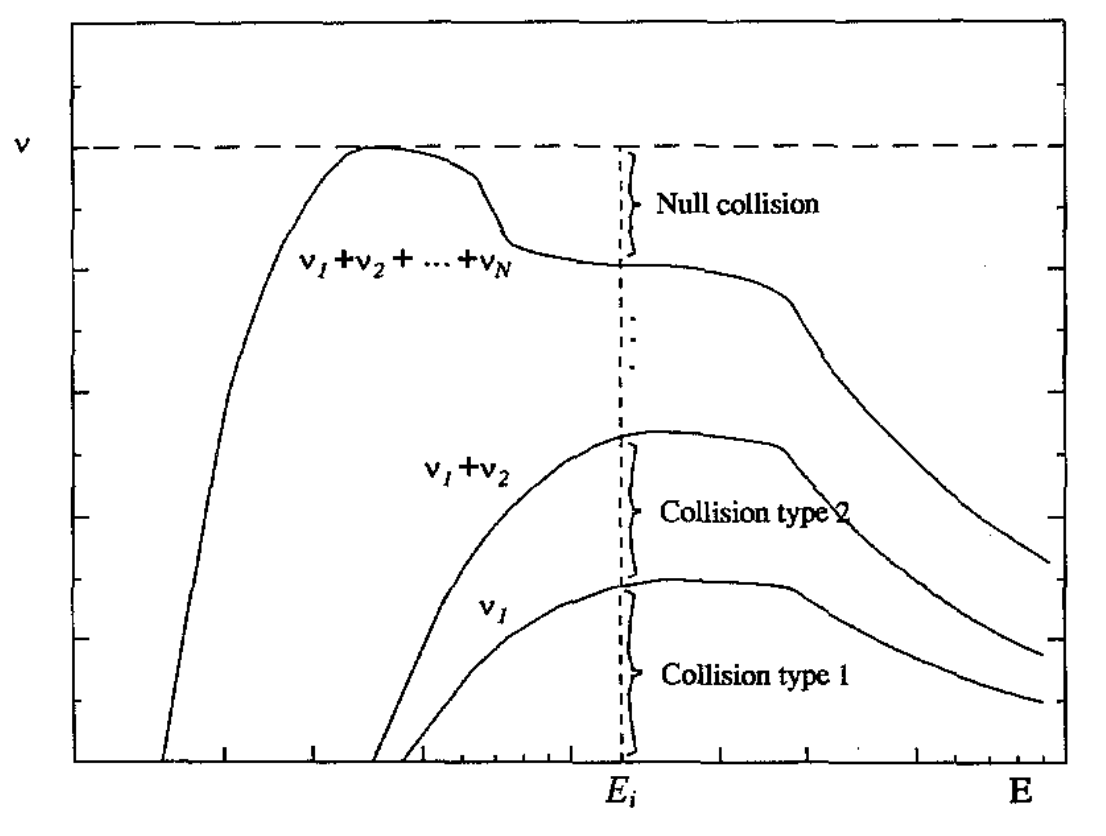
\includegraphics[width=0.6\linewidth]{particle_in_cell/figures/null_collision_option_1.png}
	\caption{Addition of null collision to produce a constant collision frequency across all energies \cite{Vahedi1995}.}
	\label{fig:null_collision}
\end{figure} 

From this, the portion of particles that should undergo a collision can be determined by the following expression \cite{Vahedi1995}:
\begin{equation}
	P(t) = 1 - e^{-\nu \Delta t}
	\label{eq:null_collisions}
\end{equation}

where $\nu$ is the maximum of the sum of all collision frequencies. This can be expressed mathematically as:
\begin{equation}
	\nu = n_g \cdot max(\sigma_{total}, v)
	\label{eq:nu}
\end{equation}
where $n_g$ is the neutral gas density (which can be assumed to be constant), $\sigma_{total}$ is the total cross section from all collisions modelled (not including the null collision), and $v$ is the relative speed between the colliding particle and the target. 

Once the number of particles that experience collisions has been determined, particles are randomly picked from the population of simulated particles. This way, the kinetic energy of only a small subset of particles from the pool will be determined, making the simulation more efficient. Once a particle has been chosen and its kinetic energy calculated, a random number between [0, 1], called $R$, is selected. This is used to determine the collision type for the particle, as a function of the value of $R$, as shown by table \ref{tb:null_collision}. 

\begin{table}[h!]
	\caption{Determining the type of collision based on the value of $R$ \cite{Vahedi1995}.}
	\vspace{5 pt}
	\centering
	\begin{tabular}{r c l c}
					  & $R$ & $\leq \nu_1/\nu$			 & Collision Type 1 \\
		$\nu_1/\nu <$ & $R$ & $\leq (\nu_1 + \nu_2)/\nu$ & Collision Type 2 \\
					  & $\vdots$ &					     & 					\\
		$(\nu_1 + \nu_2 + ... + \nu_n)/\nu <$ & $R$ &    & Null Collision   \\
	\end{tabular}
	\label{tb:null_collision}
\end{table}

If the collision type selected is a null collision, then it is treated as no collision occurred.
